\documentclass[12pt, a4paper]{article}
%{{{
% Packages{{{
  \usepackage[hmarginratio=1:1,margin=1in]{geometry}
    \linespread{1.2}
  \usepackage{graphicx}
    \graphicspath{ {./images/} }
  \usepackage[dvipsnames]{xcolor}
  \usepackage[sc]{mathpazo}
  \usepackage{microtype}
  \usepackage{fancyhdr}
  \usepackage{titling}
    \renewcommand\maketitlehooka{\null\mbox{}\vfill}
    \renewcommand\maketitlehookd{\vfill\null}
  % \usepackage{background}
  % \backgroundsetup{contents=Swapnil}

  \usepackage{listings}
    \lstset{
      frame=lrtb,
      language=HTML,
      aboveskip=15px,
      belowskip=2px,
      showstringspaces=false,
      columns=flexible,
      basicstyle={\small\ttfamily},
      xleftmargin=5px,
      xrightmargin=5px,
      breakatwhitespace=true,
      tabsize=2
    }

  \usepackage{tcolorbox}
  \usepackage[utf8]{inputenc}
%}}}

% Footer section {{{
  % Creates footer
  \pagestyle{fancy}%
  \fancyhf{}%
  \lfoot{Assignment}
  \cfoot{\emph{Swapnil}}
  \rfoot{Page \thepage}
  \renewcommand{\headrulewidth}{0pt}% Line at the head invisible
  \renewcommand{\footrulewidth}{2pt}% Line at the footer visible
% }}}

% Title {{{
  \title{\Huge{\textsc{Practical on Internet Technologies}}}
  \author{}
  \date{}
% }}}
%}}}

\begin{document}
\parindent0pt

%{{{
%Title page{{{
  \begin{titlingpage}
    \maketitle
    \thispagestyle{empty}
    %{{{
    \begin{tcolorbox}
      \textbf{\emph{Name}}: \verb+Swapnil Bhowmik+

      \textbf{\emph{Class Roll Number}}: \verb+7070+

      \textbf{\emph{University}}:

      \ \ \ \ \emph{Registration Number}: \verb+20200006768+

      \ \ \ \ \emph{Roll}: \verb+052120+

      \ \ \ \ \emph{Number}: \verb+400200086+

      \textbf{\emph{Paper Code}}: \verb+CACDSE504L+
    \end{tcolorbox}
    %}}}
  \end{titlingpage}
  \newpage
%}}}

% % ToC{{{
%   \thispagestyle{empty}
%   \tableofcontents
%   \thispagestyle{empty}
%   \vspace{2cm}
%   \begin{tabular}{@{}p{2.4in}@{}}
%   \hrulefill \\
%     \textbf{Teacher's Signature}\\
%   \end{tabular}
%   \newpage
% %}}}
%}}}


% Q1{{{
\begin{tcolorbox}
  \section{Write a program in HTML of the following:}
  \begin{enumerate}
    \item{To insert two image files.}
    \item{To use hyperlink to connect two pages.}
    \item{To insert three headings of different sizes.}
  \end{enumerate}
\end{tcolorbox}
\subsection*{Date of Experiment:}
07/11/2022
\subsection*{Objective:}
Using html we have to demonstrate how to insert image, how to create hyper link, how to insert heading of different sizes in a web page.

\subsection*{Program:}
\begin{lstlisting}
<html>
  <head>
    <title>
      Question 1
    </title>
  </head>
  <body>
    <a href="secondpage.html">Next Page</a><br><hr>
    <h1>Images</h1>
    <img src="img/picture1.png" width="500px" alt="Man and Women" /><br>
    <img src="img/picture2.png" width="500px" alt="Woman" />
  </body>
</html>
\end{lstlisting}
\newpage
\subsection*{Output:}
\begin{figure}[h]
  \centering
  
\includegraphics[height=0.45\textheight]{1}
  \caption{First Page}
\end{figure}
\begin{figure}[h]
  \centering
  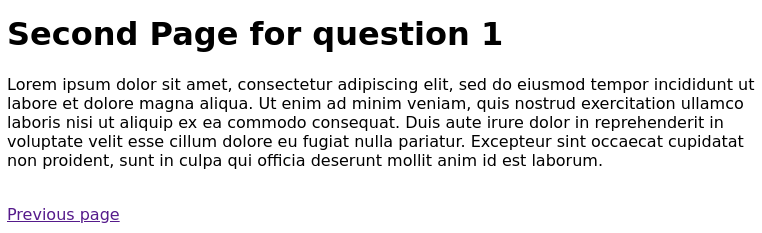
\includegraphics[width=\textwidth]{2}
  \caption{Second Page}
\end{figure}

\pagebreak
%}}}

% Q2{{{
\begin{tcolorbox}
  \section{Write a program in HTML to display the following table}
  \hskip28pt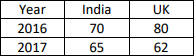
\includegraphics{3}
\end{tcolorbox}
\subsection*{Date of Experiment:}
07/11/2022
\subsection*{Objective:}
Demonstrate how to insert a table in a web page using html.

\subsection*{Program:}
\begin{lstlisting}
<html>
  <head>
    <title>
      Table
    </title>
  </head>
  <body>
    <table border="1px">
      <th>Year</th> <th>India</th> <th>UK</th>
      <tr> <td>2016</td> <td>70</td> <td>80</td> </tr>
      <tr> <td>2017</td> <td>65</td> <td>62</td> </tr>
    </table>
  </body>
</html>
\end{lstlisting}
\subsection*{Output:}
\begin{figure}[ht]
  \centering
  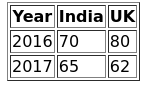
\includegraphics{4}
\end{figure}

\pagebreak
%}}}

% Q3{{{
\begin{tcolorbox}
  \section{Write a program in JavaScript to multiply two numbers using two text boxes, one command button and on-click event handler}
\end{tcolorbox}
\subsection*{Date of Experiment:}
07/11/2022
\subsection*{Objective:}
Multiply two numbers using two text boxes, one command button and on-click event handler.

\subsection*{Program:}
\begin{lstlisting}
<html>
  <head>
    <title>
      Question 3
    </title>
  </head>
  <body>
    <script>
    function multiply() {
      n1 = document.getElementById("frst").value;
      n2 = document.getElementById("scnd").value;
      document.getElementById("result").innerHTML=n1*n2;
    }
  </script>
    Enter 1st number: <input type="text" id="frst" /> <br>
    Enter 2nd number: <input type="text" id="scnd" /> <br>
    <input type="button" value="Calculate" onclick="multiply()" /> 
    <h1 id="result"></h1>
  </body>
</html>
\end{lstlisting}
\pagebreak
\subsection*{Output:}
\begin{figure}[ht]
  \centering
  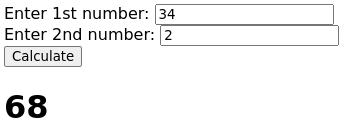
\includegraphics{5}
\end{figure}

\pagebreak
%}}}

% Q4 {{{
\begin{tcolorbox}
  \section{Write a HTML program to input name, roll no, semester, department \& year of a student and display the output in a tabular form}
\end{tcolorbox}
\subsection*{Date of Experiment:}
08/11/2022
\subsection*{Objective:}
Using HTML we have to input name, roll no, semester, department \& year of a student and display the output in a tabular form.

\subsection*{Program:}
\begin{lstlisting}
<html>
  <head>
    <title>Tabular form
    </title>
  </head>
  <body>
    <table>
      <tr>
        <th>Name</th> <th>Roll no</th> <th>Semester</th>
        <th>Department</th> <th>Year</th>
      </tr>
      <tr>
        <td> <input type="text"> </td>
        <td> <input type="text"> </td>
        <td> <input type="text"> </td>
        <td> <input type="text"> </td>
        <td> <input type="text"> </td>
      </tr>
    </table>
  </body>
</html>
\end{lstlisting}
\pagebreak
\subsection*{Output:}
\vskip10pt
\begin{figure}[ht]
  \centering
  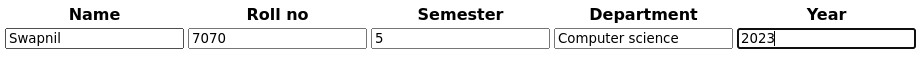
\includegraphics[width=\textwidth]{6}
\end{figure}

\pagebreak
%}}}

% Q5 {{{
\begin{tcolorbox}
  \section{Write a program to design a database of a student with attributesname, roll no, contact no, DOB, department, year in XML.}
\end{tcolorbox}
\subsection*{Date of Experiment:}
10/11/2022
\subsection*{Objective:}
Using XML we have to design a database of a student with attributes-name, roll no, contact no, DOB, department, year.

\subsection*{Program:}
\begin{lstlisting}
<student>
	<name>
		<s_name>Masuk</s_name>
		<s_name>Moinak</s_name>
		<s_name>Swapnil</s_name>
		<s_name>Srijani</s_name>
	</name>
	<roll>
		<s_roll>1001</s_roll>
		<s_roll>1002</s_roll>
		<s_roll>1003</s_roll>
		<s_roll>1004</s_roll>
	</roll>
	<contact>
		<c_no>99000000</c_no>
		<c_no>95555000</c_no>
		<c_no>96500000</c_no>
		<c_no>94500000</c_no>
	</contact>
	<dob>
		<birth>10-05-2000</birth>
		<birth>23-03-2001</birth>
		<birth>13-09-2002</birth>
		<birth>23-06-2002</birth>
	</dob>
	<dep>
		<dep_n>Computer Application</dep_n>
		<dep_n>Computer Application</dep_n>
		<dep_n>Computer Application</dep_n>
		<dep_n>Computer Application</dep_n>
	</dep>
	<yrs>
		<y_n>2023</y_n>
		<y_n>2023</y_n>
		<y_n>2023</y_n>
		<y_n>2023</y_n>
	</yrs>
</student>
\end{lstlisting}
\pagebreak
\subsection*{Output:}
\vskip10pt
\begin{figure}[h]
  \centering
  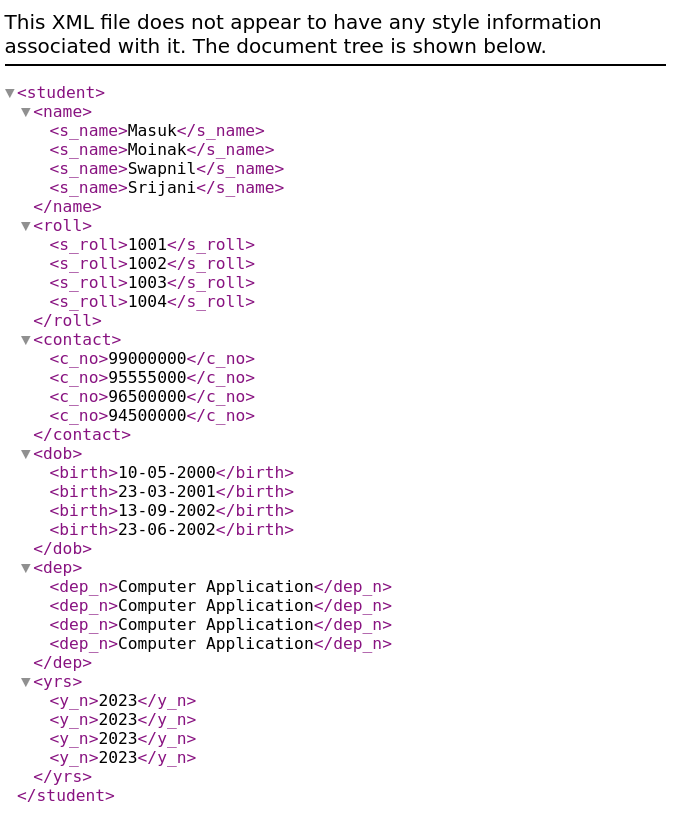
\includegraphics[width=0.9\textwidth]{7}
\end{figure}

\pagebreak
%}}}

% Q6 {{{
\begin{tcolorbox}
  \section{Write a JavaScript program to display a character string in the reverse order.}
\end{tcolorbox}
\subsection*{Date of Experiment:}
10/11/2022
\subsection*{Objective:}
Display a character string in the reverse order using JavaScript.

\subsection*{Program:}
\begin{lstlisting}
<html>
  <head>
    <title>
      JavaScript program to display a character string in the reverse order.
    </title>
  </head>
  <body>
    <script>
      function textrev() {
        let concatArr = "";
        input = document.getElementById("textinput").value;
        for(var i = input.length-1; i >= 0; i--) {
          concatArr = concatArr + input[i];
        }
        document.getElementById("output").innerHTML = concatArr;
      }
    </script>
    Enter the text: 
    <input type="text" id="textinput" />
    <input type="button" id="button" onclick="textrev()" value="Reverse" />
    <h1 id="output">
    </h1>
  </body>
</html>
\end{lstlisting}
\pagebreak
\subsection*{Output:}
\vskip10pt
\begin{figure}[h]
  \centering
  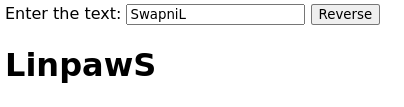
\includegraphics{8}
\end{figure}

\pagebreak
%}}}

% Q7 {{{
\begin{tcolorbox}
  \section{Write a JavaScript code to count the number of digits in a given number.}
\end{tcolorbox}
\subsection*{Date of Experiment:}
14/11/2022
\subsection*{Objective:}
Count the number of digits in a given number using JavaScript.

\subsection*{Program:}
\begin{lstlisting}
<html>
  <head>
    <title>
      Write a JavaScript code to count the number of digits in a given number.
    </title>
  </head>
  <body>
  <script>
    function numcount() {
      let count = 0;
      input = document.getElementById("numinput").value;
      document.getElementById("output").innerHTML = input.length;
    }
  </script>
  Enter the number: <input type="text" id="numinput" />
    <input type="button" id="button" onclick="numcount()" value="Count" />
    <h1 id="output"></h1>
  </body>
</html>
\end{lstlisting}
\subsection*{Output:}
\begin{figure}[h]
  \centering
  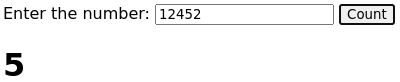
\includegraphics{9}
\end{figure}

\pagebreak
%}}}

% Q8 {{{
\begin{tcolorbox}
  \section{Write a HTML to design a form that has the following attribute Name, Address, E-mail, Contact Number.}
\end{tcolorbox}
\subsection*{Date of Experiment:}
14/11/2022
\subsection*{Objective:}
Create a HTML form that has the following attribute Name, Address, E-mail, Contact Number.

\subsection*{Program:}
\begin{lstlisting}
<html>
  <head>
    <title>Basic Form
    </title>
  </head>
  <body>
    <form>
      <div>
        <label for="name">Name:
        </label>
        <input type="text" required>
      </div>
      <div >
        <label for="name">Address:
        </label>
        <input type="text" required>
      </div>
      <div >
        <label for="email">Email:
        </label>
        <input type="email" required>
      </div>
      <div >
        <label for="number"> Contect Number 
          <span class="clue">(optional):</span>
        </label>
        <input type="tel">
      </div>
      <div>
        <button type="submit">Submit
        </button>
        <button type="reset">Reset
        </button>
      </div>
    </form>
  </body>
</html>
\end{lstlisting}
\subsection*{Output:}
\vskip10pt
\begin{figure}[h]
  \centering
  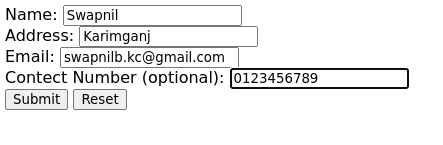
\includegraphics{10}
\end{figure}

\pagebreak
%}}}

% Q9 {{{
\begin{tcolorbox}
  \section{Write a code in HTML to}
  \begin{enumerate}
    \item Layout pages using tables;
    \item Create navigation bars;
  \end{enumerate}
\end{tcolorbox}
\subsection*{Date of Experiment:}
25/11/2022
\subsection*{Objective:}
Create layout pages using tables and also we have to a navigation bars.

\subsection*{Program:}
\subsubsection*{1. Layout pages using tables:}
\begin{lstlisting}
<html>
  <head>
    <title>Basic HTML Layout using Tables
    </title>
  </head>
  <body>
    <table width="100%" border="1" align="center">
      <tr>
        <td colspan="2" bgcolor="forestgreen">
          <h1>Website Title or Header
          </h1>
        </td>
      </tr>
      <tr valign="top">
        <td bgcolor="skyblue" width="25%">
          This is section area...
        </td>
        <td bgcolor="red" width="60%" height="200">
          This is the main content area.
        </td>
      </tr>
      <tr>
        <td colspan="2" bgcolor="lightblue" align="center">
          Created by swapnil
        </td>
      </tr>
    </table>
  </body>
</html>
\end{lstlisting}
\subsubsection*{2. Create navigation bars:}
\begin{lstlisting}
<html>
  <head>
    <title>Navigation Bar
    </title>
    <style type="text/css">
      header {
        background-color: black;
        position: fixed;
        left: 0;
        right: 0;
        top: 10px;
        height: 30px;
        align-items: center;
        display: inline;
      }
      header * {
        display: inline;
      }
      header li {
        margin: 20px;
      }
      header li a {
        color: white;
        text-decoration: none;
      }
    </style>
  </head>
  <body>
    <header>
      <nav>
        <ul>
          <li> <a href="./InsertImg.html">Home</a> </li>
          <li> <a href="./layoutP.html">About</a> </li>
          <li> <a href="./Form.html">Contact</a> </li>
          <li> <a href="#">Terms of use</a> </li>
        </ul>
      </nav>
    </header>
  </body>
</html>
\end{lstlisting}
\subsection*{Output:}
\vskip10pt
\setcounter{figure}{0}
\begin{figure}[h]
  \centering
  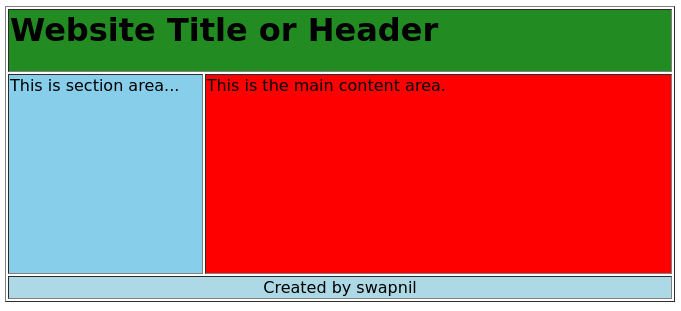
\includegraphics[width=\textwidth]{11}
  \caption{Layout pages using tables}
\end{figure}
\begin{figure}[h]
  \centering
  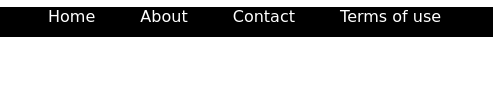
\includegraphics[width=\textwidth]{12}
  \caption{Create navigation bars}
\end{figure}

\pagebreak
%}}}

% Q10 {{{
\begin{tcolorbox}
  \section{Write a JavaScript code to pick a phrase from an array of sent}
\end{tcolorbox}
\subsection*{Date of Experiment:}
25/11/2022
\subsection*{Objective:}
Pick a phrase from an array of sentences using JavaScript.

\subsection*{Program:}
\begin{lstlisting}
<html>
  <body>
    <script>
      var keywords = ["Moinak", "Masuk", "Srijani", "Swapnil"];
      var sentence = ["Hello, I am Swapnil and my friends are Masuk, Moinak
                        and Srijani"];
      const matched = [];
      for (var index = 0; index < sentence.length; index++) {
        for (var outerIndex = 0; outerIndex < keywords.length; outerIndex++) {
          if (sentence[index].includes(keywords[outerIndex])) {
            matched.push(keywords[outerIndex]);
          }
        }
      }
      document.write("The matched elements are:-"+matched);
    </script>
  </body>
</html>
\end{lstlisting}
\subsection*{Output:}
\vskip10pt
\setcounter{figure}{0}
\begin{figure}[h]
  \centering
  
\includegraphics{13}
\end{figure}

\pagebreak
%}}}

% Q11 {{{
\begin{tcolorbox}
  \section{Write a JavaScript to show event on button and list.}
\end{tcolorbox}
\subsection*{Date of Experiment:}
28/11/2022
\subsection*{Objective:}
Show event on button and list using JavaScript.

\subsection*{Program:}
\begin{lstlisting}
<html>
  <head>
    <title> Event 
    </title>
  </head>
  <body>
    <ul>
      <li > 
        <button onclick="alert('Hello World')">Click me.
        </button> 
      </li>
    </ul>
  </body>
</html>
\end{lstlisting}
\subsection*{Output:}
\setcounter{figure}{0}
\begin{figure}[h]
  \centering
  
\includegraphics{14}\vskip10pt

  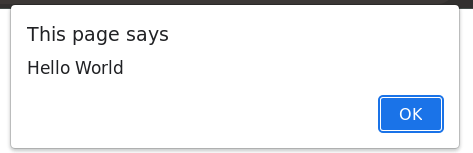
\includegraphics[width=0.7\textwidth]{15}
\end{figure}

\pagebreak
%}}}

% Q12{{{
\begin{tcolorbox}
  \section{Write a program that prints a table of numbers from 5 to 15 and their squares and cubes using alert.}
\end{tcolorbox}
\subsection*{Date of Experiment:}
28/11/2022
\subsection*{Objective:}
Print a table of numbers from 5 to 15 and their squares and cubes using alert.

\subsection*{Program:}
\begin{lstlisting}
<html>
  <head>
    <title>
      Write a program that prints a table of numbers from 5 to 15 and their
      squares and cubes using alert.
    </title>
  </head>
  <body>
    <input type="button" id="output" value="Click the button" />
    <script>
      function printtab() {
        var out = "";
        for (i = 5; i <= 15; i++) {
          alert("square of "+i+" is "+i*i+" and the cube is "+i*i*i);
        }
      }
      document.getElementById("output").addEventListener("click", printtab);
    </script>
  </body>
</html>
\end{lstlisting}
\pagebreak
\subsection*{Output:}
\begin{figure}[h]
  \centering
  
\includegraphics{16}
  \vskip30pt
  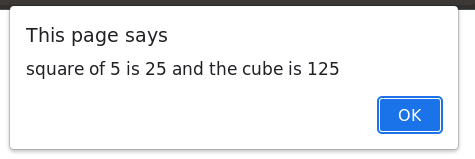
\includegraphics[width=0.45\textwidth]{17}
  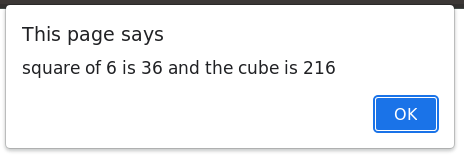
\includegraphics[width=0.45\textwidth]{18}
  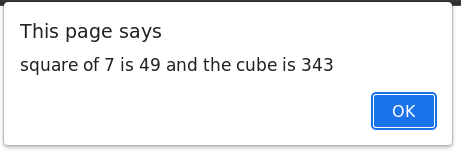
\includegraphics[width=0.45\textwidth]{19}
  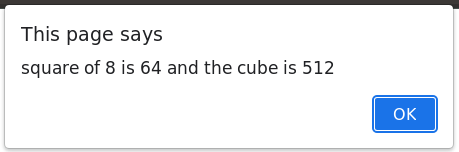
\includegraphics[width=0.45\textwidth]{20}
  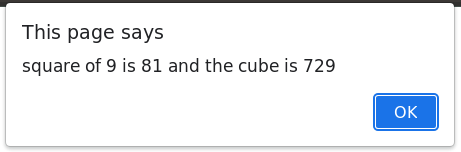
\includegraphics[width=0.45\textwidth]{21}
  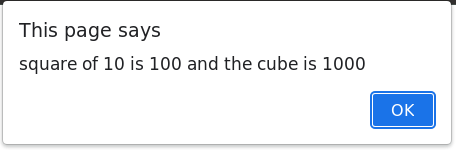
\includegraphics[width=0.45\textwidth]{22}
  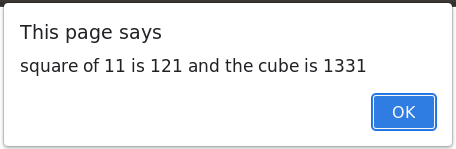
\includegraphics[width=0.45\textwidth]{23}
  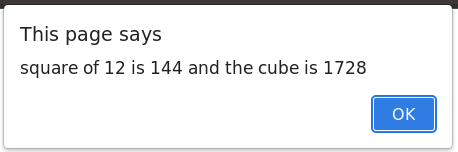
\includegraphics[width=0.45\textwidth]{24}
  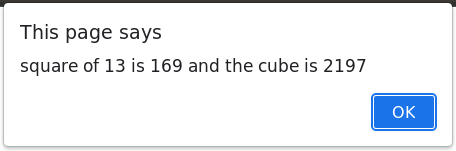
\includegraphics[width=0.45\textwidth]{25}
  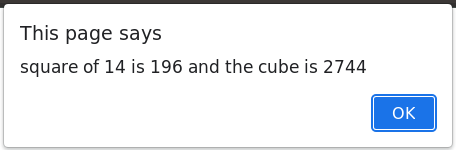
\includegraphics[width=0.45\textwidth]{26}
  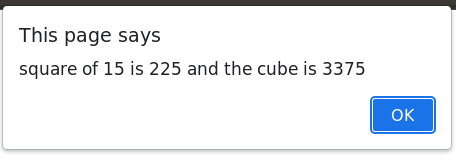
\includegraphics[width=0.45\textwidth]{27}
\end{figure}

\pagebreak
%}}}

% Q13{{{
\begin{tcolorbox}
  \section{Write a program that prints the largest of three number.}
\end{tcolorbox}
\subsection*{Date of Experiment:}
 01/12/2022
\subsection*{Objective:}
Print the largest of three number using JavaScript.

\subsection*{Program:}
\begin{lstlisting}
<html>
  <head>
    <title>
      Print the largest of three number using JavaScript.
    </title>
  </head>

  <body>
    <script type="text/javascript">
      function greatest() {
        var n1, n2, n3, grt;
        n1 = parseInt(document.getElementById("no1").value);
        n2 = parseInt(document.getElementById("no2").value);
        n3 = parseInt(document.getElementById("no3").value);
        if (n1 > n2 && n1 > n3)
          grt = n1;
        else if (n2 > n1 && n2 > n3)
          grt = n2;
        else
          grt = n3;
        document.write("The Largest number is " + grt);
      }
    </script>
    Enter First Number 
    <br>
    <input type="text" id="no1">
    <br>
    Enter Second Number 
    <br>
    <input type="text" id="no2">
    <br>
    Enter Third Number 
    <br>
    <input type="text" id="no3">
    <br>
    <br>
    <input type="button" value="Find the largest" onclick="greatest()">
  </body>
</html>
\end{lstlisting}
\subsection*{Output:}
\begin{figure}[h]
  \centering
  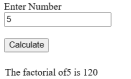
\includegraphics[width=0.3\textwidth]{43}
\end{figure}

\pagebreak
%}}}

% Q14{{{
\begin{tcolorbox}
  \section{Write a program that finds the factorial of a number n.}
\end{tcolorbox}
\subsection*{Date of Experiment:}
01/12/2022
\subsection*{Objective:}
Find the factorial of a number n.

\subsection*{Program:}
\begin{lstlisting}
<html>
  <head>
    <title>
      Question Number 3
    </title>
  </head>
  <body>
    <script type="text/javascript">
      function factorial() {
        var n, f;
        f = 1;
        n = parseInt(document.getElementById("num").value);
        for (var i = 1; i <= n; i++) {
          f = f * i;
        }
        document.write("The factorial of" + n + " is " + f);
      }
    </script>
    Enter Number
    <br>
    <input type="text" id="num">
    <br>
    <br>
    <input type="button" value="Calculate" onclick="factorial()">
  </body>
</html>
\end{lstlisting}
\pagebreak
\subsection*{Output:}
\begin{figure}[h]
  \centering
  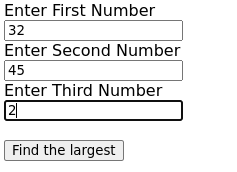
\includegraphics{28}
  \caption{Input}
\end{figure}

\begin{figure}[h]
  \centering
  
\includegraphics{29}
  \caption{Result}
\end{figure}

\pagebreak
%}}}

% Q15{{{
\begin{tcolorbox}
  \section{Enter a list of positive numbers terminated by Zero. Find the sum and average of these numbers.}
\end{tcolorbox}
\subsection*{Date of Experiment:}
14/12/2022
\subsection*{Objective:}
Enter a list of positive numbers terminated by Zero also we have to the sum and average of these numbers using JavaScript.

\subsection*{Program:}
\begin{lstlisting}
<html lang="en">

  <head>
    <title>
      Question Number 4
    </title>
  </head>

  <body>
    <input type="button" value="Sum and Average" onclick="average()">
    <script>
      function average() {
        var sum = 0;
        var num;
        var x, i;
        for (i=1; ; i++){
          num = prompt("Enter array Element terminated by Zero: ");
          var x = parseInt(num);
          sum += x;
          if (num == 0) {
            var av = (sum / i);
            document.write("Sum is: "+sum+" and Average is: "+av);
            break;
          }
        }
      }
    </script>
  </body>
</html>
\end{lstlisting}
\subsection*{Output:}
\setcounter{figure}{0}
\begin{figure}[h]
  \centering
  
\includegraphics{30}
  \vskip40pt

  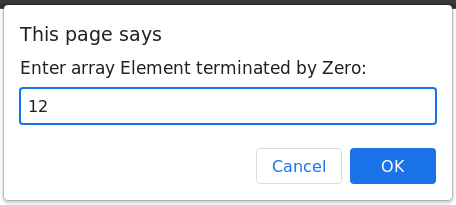
\includegraphics[width=0.45\textwidth]{31}
  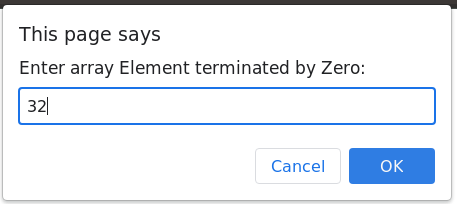
\includegraphics[width=0.45\textwidth]{32}
  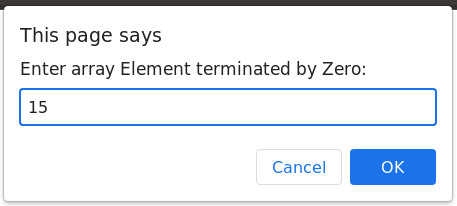
\includegraphics[width=0.45\textwidth]{33}
  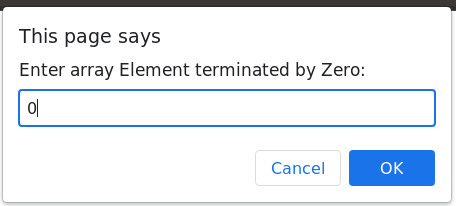
\includegraphics[width=0.45\textwidth]{34}
  \caption{Input}
\end{figure}

\begin{figure}[h]
  \centering
  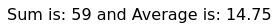
\includegraphics{35}
  \caption{Result}
\end{figure}

\pagebreak
%}}}

% Q16{{{
\begin{tcolorbox}
  \section{A person deposits Rs 1000 in a fixed account yielding 5\% interest. Compute the amount in the account at the end of each year for n years.}
\end{tcolorbox}
\subsection*{Date of Experiment:}
14/12/2022
\subsection*{Objective:}
A person deposits Rs 1000 in a fixed account yielding 5\% interest. Compute the amount in the account at the end of each year for n years.

\subsection*{Program:}
\begin{lstlisting}
<html>
  <head>
    <title>
      Question 5
    </title>
  </head>
  <body>
    Enter number of years::::::::::
    <br>
    <input id="n">
    <input type="button" value="Compute intrst and amount " onclick="avg()">
    <script>
      function avg() {
        var t = parseInt(document.getElementById("n").value);
        for (var i = 1; i <= t; i++) {
          var interest = parseInt((1000 * 5 * i) / 100);
          document.write("Interest after "+i+" year is :<b>"+interest+"</b>
                            and total amount after " + i + " years" + " becomes:
                            <b>" + (interest + 1000) + "</b><br>")
        }
      }
    </script>
  </body>
</html>
\end{lstlisting}
\subsection*{Output:}
\setcounter{figure}{0}
\begin{figure}[h]
  \centering
  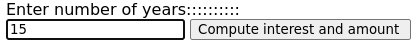
\includegraphics{36}
  \caption{Input}
\end{figure}

\begin{figure}[h]
  \centering
  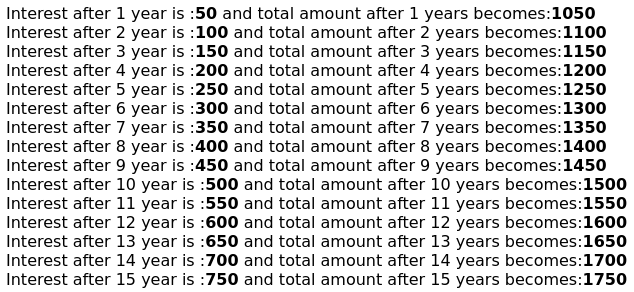
\includegraphics[width=\textwidth]{37}
  \caption{Result}
\end{figure}

\pagebreak
%}}}

% Q17{{{
\begin{tcolorbox}
  \section{Read n numbers. Count the number of negative numbers, positive numbers and zeros in the list.}
\end{tcolorbox}
\subsection*{Date of Experiment:}
14/12/22
\subsection*{Objective:}
Count the number of negative numbers, positive numbers and zeros in the list.

\subsection*{Program:}
\begin{lstlisting}
<html>
  <body>
    Enter the size of the list : <input id="n1"><br>
    <input type="button" value="Count +,-,0" onclick="avg()">
    <script type="text/javascript">
      function counter(ar) {
        var array1 = [0, 0, 0];
        for (var i = 0; i < ar.length; i++) {
          switch (ar[i] < 0) {
            case true: array1[0]++;
              break;
            case false:
              if (ar[i] == 0) array1[1]++;
              else array1[2]++;
              break;
            default: break;
          }
        } return (array1);
      }
      function avg() {
        var ar1 = [];
        var n = parseInt(document.getElementById("n1").value);
        var ar = [];
        var size = n;
        for (var a = 0; a < size; a++) {
          ar[a] = prompt("Enter the"+(a+1)+"st elements of an array");
        }
        document.write(" Elements are : "+"<br>");
        for (var j = 0; j < ar.length; j++) {
          document.write(ar[j] + '<br>')
        }
        document.write("______________________________________" + "<br>");
        ar1 = counter(ar);
        document.write("No of Negative Elements are : "+ar1[0]+"<br>");
        document.write("No of Zero  Elements are : "+ar1[1]+"<br>");
        document.write("No of Positive Elements are : "+ar1[2]+"<br>");
      } 
    </script>
  </body>
</html>

\end{lstlisting}
\subsection*{Output:}
\setcounter{figure}{0}
\begin{figure}[h]
  \centering
  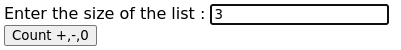
\includegraphics{38}
  \vskip10pt

  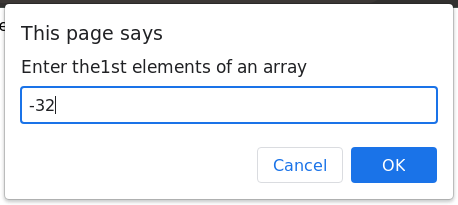
\includegraphics[width=0.38\textwidth]{39}\hskip10pt
  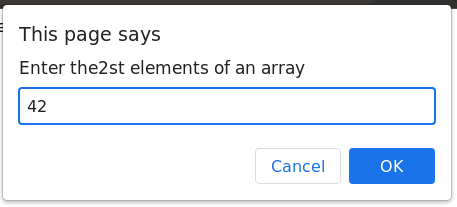
\includegraphics[width=0.38\textwidth]{40}
  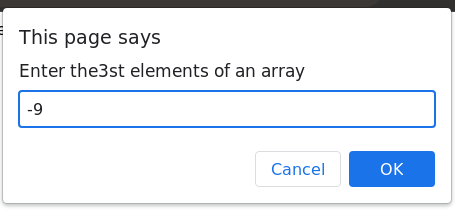
\includegraphics[width=0.38\textwidth]{41}
  \caption{Input}
\end{figure}

\begin{figure}[h]
  \centering
  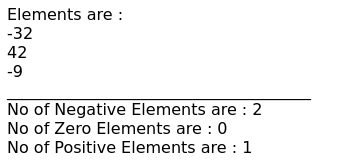
\includegraphics{42}
  \caption{Result}
\end{figure}

\pagebreak
%}}}

\end{document}
